\documentclass[border=10pt]{standalone}
\usepackage{tikz}
\usetikzlibrary{shadings, calc, decorations.markings}
\tikzset{->-/.style={decoration={
			markings,
			mark=at position #1 with {\arrow{>}}},postaction={decorate}},
	->-/.default=0.5,
}
\begin{document}
	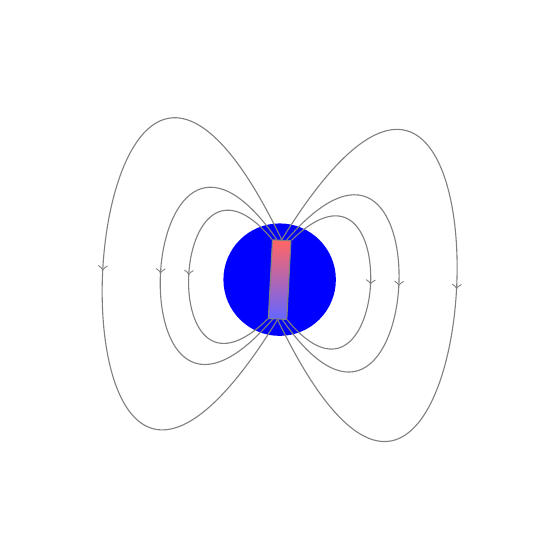
\begin{tikzpicture}
		\def\angle{87}% change this to rotate the magnet
		\path [use as bounding box] (-3.2,-3.2) rectangle (3.2,3.2);
		%\draw[very thin, gray!50] (-3,-3) grid (3,3);
		\draw[thick, color=blue, fill=blue] (0, 0) circle (0.7);
		\begin{scope}[gray,text=black, rotate=\angle]
			\node[draw, left color=blue!60,right color=red!60,
			rotate=\angle, shading angle=90+\angle, minimum width=1cm,
			]
			at (0,0) (I) {};
			\draw[->-] (I.north east) .. controls (2,1.5) and (-2,1.5) ..  (I.north west);
			\coordinate (n1) at ($ (I.north east)!0.5!(I.east) $);
			\coordinate (s1) at ($ (I.north west)!0.5!(I.west) $);
			\draw[->-] (n1) .. controls (3, 2) and (-3, 2) .. (s1);
			\draw[->-] (I.east) .. controls (6,3) and (-6,3) .. (I.west);
			\draw[->-] (I.south east) .. controls (2,-1.5) and (-2,-1.5) ..  (I.south west);
			\coordinate (n2) at ($ (I.south east)!0.5!(I.east) $);
			\coordinate (s2) at ($ (I.south west)!0.5!(I.west) $);
			\draw[->-] (n2) .. controls (3, -2) and (-3, -2) .. (s2);
			\draw[->-] (I.east) .. controls (6,-3) and (-6,-3) .. (I.west);
		\end{scope}
	\end{tikzpicture}
\end{document}

%
%\documentclass{standalone}
%\usepackage{tikz}
%\usetikzlibrary{calc}
%\usetikzlibrary{decorations.markings}
%
%\tikzstyle directed=[postaction={decorate,decoration={markings, % arrows on the field lines
%		mark=at position .1 with {\arrowreversed[scale=1.5]{stealth}},
%		mark=at position .9 with {\arrowreversed[scale=1.5]{stealth}}}}]
%\tikzstyle tangent=[postaction={decorate,decoration={markings, % Tangent to the field line
%		mark=at position .7 with {\draw[ultra thick,stealth-,green!60!black,solid](-10pt,0)--(10pt,0)node[above]{$\vec{B}$};}}}]
%\tikzstyle fLines=[thick,dashed,directed,tangent]
%
%\begin{document}
%	\begin{tikzpicture}
%		\def\lmag{1.5}  % length of magnet
%		\def\wmag{0.4}  % thickness of magnet
%		\def\nc{5}      % no. of lines = 2*\nc+1
%		
%		\begin{scope}
%			\draw[thick, color=blue, fill=blue] (0, 0) circle (1);
%			\coordinate (A) at (-\lmag/2,\wmag/2);
%			\coordinate (B) at (\lmag/2,-\wmag/2);
%			
%			\clip (-5,-4) rectangle (5,4);
%			\foreach \r in {1,...,\nc}{
%				\draw[fLines]($(A)-(0,0.5*\r*\wmag/\nc)$) arc(({270-asin(\lmag/(2*\r))}):({-90+asin(\lmag/(2*\r))}):\r);
%				\draw[fLines]($(B)+(0,0.5*\r*\wmag/\nc)$) arc(({90-asin(\lmag/(2*\r))}):({-270+asin(\lmag/(2*\r))}):\r); }
%			\draw[fLines] (-\lmag/2,0) -- ++(-6,0);
%			\draw[fLines] (\lmag/2,0) ++(6,0)--(\lmag/2,0);
%		\end{scope}
%	\end{tikzpicture}
%\end{document}